% % =============================================================================
% % esempi_latex.tex  -  Riferimento rapido ai comandi LaTeX piu' utili
% %
% % NOTA: Questo file NON fa parte della tesi finale.
% %       Viene incluso nel documento solo durante la stesura come riferimento.
% %       Prima della stampa, commenta la riga % % =============================================================================
% % esempi_latex.tex  -  Riferimento rapido ai comandi LaTeX piu' utili
% %
% % NOTA: Questo file NON fa parte della tesi finale.
% %       Viene incluso nel documento solo durante la stesura come riferimento.
% %       Prima della stampa, commenta la riga % % =============================================================================
% % esempi_latex.tex  -  Riferimento rapido ai comandi LaTeX piu' utili
% %
% % NOTA: Questo file NON fa parte della tesi finale.
% %       Viene incluso nel documento solo durante la stesura come riferimento.
% %       Prima della stampa, commenta la riga % % =============================================================================
% % esempi_latex.tex  -  Riferimento rapido ai comandi LaTeX piu' utili
% %
% % NOTA: Questo file NON fa parte della tesi finale.
% %       Viene incluso nel documento solo durante la stesura come riferimento.
% %       Prima della stampa, commenta la riga \input{capitoli/esempi_latex}
% %       nel file tesi.tex.
% % =============================================================================

% \section{Immagini}
% Quando usi \texttt{figure}, ricordati il modificatore di posizione tra quadre:
% \texttt{H} significa esattamente nel punto dove si trova nel file .tex (consigliato).

% \begin{figure}[H]
%     \centering
%     % Se metti solo una delle due dimensioni, l'altra scala in automatico.
%     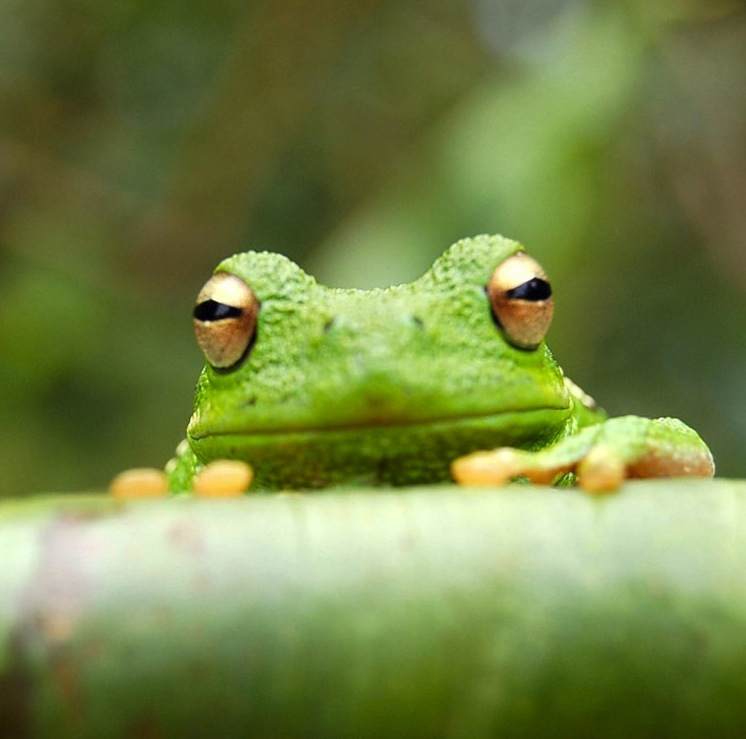
\includegraphics[height=6cm, width=8cm]{img/frog.jpg}
%     \caption{Caption (questo viene scritto nell'indice delle figure)}
%     % La label serve per riferirti all'immagine piu' avanti nel testo: \cref{fig:frog}
%     \label{fig:frog}
% \end{figure}

% \section{Tabelle}
% \subsection{Tabella semplice}
% Nota il modificatore \texttt{[H]}, la caption e la label.

% \begin{table}[H]
%     \centering
%     \begin{tabular}{|c|c|}
%     \hline
%         \textbf{Pratiche agili} & \textbf{Studenti}  \\ \hline
%         Sprint planning & 73  \\ \hline
%         Pair programming & 73  \\ \hline
%         Retrospettiva & 48  \\ \hline
%     \end{tabular}
%     \caption{Tabella semplice (anche questo viene scritto nell'indice delle tabelle)}
%     \label{tab:simple}
% \end{table}

% \subsection{Tabelle avanzate}
% Con \texttt{multirow} puoi fare righe piu' grandi del normale.

% \begin{table}[H]
%     \centering
%     \begin{tabular}{|c|c|c|c|c|}
%     \hline
%         \textbf{Team} & \textbf{LoC ver.} & \textbf{LoC svil.} & \textbf{Ore svil.} & \textbf{LoC/h}  \\ \hline
%         \multirow{2}*{1} & 1148 & m: 888  & m: 40 & 22\cr & Diff: $-$1852 & $\sigma$: 371 & $\sigma$: 27 & \\ \hline
%         \multirow{2}*{2} & 1858 & m: 1404 & m: 65 & 22\cr & Diff: $-$448  & $\sigma$: 1222 & $\sigma$: 78 & \\ \hline
%         \multirow{2}*{3} & 1640 & m: 1400 & m: 96 & 15\cr & Diff: $-$2810 & $\sigma$: 1417 & $\sigma$: 41 & \\ \hline
%     \end{tabular}
%     \caption{Tabella con multirow}
%     \label{tab:avanz}
% \end{table}

% \subsubsection{Tabelle girate}
% Se usi \texttt{landscape} la tabella viene girata (utile per tabelle molto larghe).
% \begin{landscape}
% \begin{table}[H]
%     \centering
%     \begin{tabular}{|c|c|}
%     \hline
%         \textbf{Numero} & \textbf{\#}  \\ \hline
%         UNO & 1  \\ \hline
%         DUE & 2  \\ \hline
%         TRE & 3  \\ \hline
%     \end{tabular}
%     \caption{Tabella girata}
%     \label{tab:girata}
% \end{table}
% \end{landscape}

% \section{Grafici con TikZ}
% Puoi creare grafici con \texttt{tikzpicture}.
% Tutorial completo: \url{https://tikz.dev/}

% % Esempio: assi cartesiani con range ragionevole (max x=10 per evitare overfull)
% \begin{tikzpicture}
%   \draw[->] (-0.5,0) -- (10,0) node[right] {$x$};
%   \draw[->] (0,-0.5) -- (0,5) node[above] {$y$};
%   \foreach \x in {1,2,...,9}
%     \draw (\x,-0.1) -- (\x,0.1) node[below] {\tiny\x};
%   \foreach \y in {1,2,3,4}
%     \draw (-0.1,\y) -- (0.1,\y) node[left] {\tiny\y};
%   \fill (0,0) circle[radius=2pt];
%   % Esempio di curva:
%   \draw[blue, thick, domain=0:9, samples=100] plot (\x, {0.5*\x});
% \end{tikzpicture}

% \section{Import di altri file .tex}
% Molto utile per capitoli separati:
% \begin{verbatim}
% \input{capitoli/capitolo1_contesto}
% \end{verbatim}

% \section{Math mode}
% Inline: $5 \times \alpha = 3\lambda$

% Display:
% \[ \frac{\sum_{i=1}^{n} 3i\theta}{12k^2 \times 7} \]

% Numerata (con label):
% \begin{equation}
%     \frac{1}{2} \times A_{bcd} \times E^{fgh}
%     \label{eq:esempio}
% \end{equation}

% \section{URL e note a pie' di pagina}
% Per mettere un link usa \verb|\url{}|: \url{https://wikipedia.org}

% Per note a pie' di pagina usa \verb|\footnote{}|\footnote{Tipo questa.}

% \section{Code snippet}
% \begin{lstlisting}[language=C, caption={Hello World in C}, label={lst:helloC}]
% #include <stdio.h>

% int main(void) {
%     printf("Hello World\n");
%     return 0;
% }
% \end{lstlisting}

% \section{Verbatim}
% \begin{verbatim}
%     Qui puoi scrivere

%     come      vuoi
%     e viene tutto
% scritto monospaziato
% \end{verbatim}

% \section{Riferimenti incrociati}
% Le label servono per riferirti ad altre parti del testo.
% Esempio: ``vedi \cref{chap:intro}''.\\
% Con \texttt{cleveref} ottieni automaticamente la dicitura corretta:
% \cref{chap:intro}, \cref{tab:simple}, \cref{fig:frog}, \cref{eq:esempio}.

% \section{Citazioni}
% Per citare usa \verb|\cite{}| con la chiave del file \texttt{refs.bib}.
% Esempio:
% \begin{verbatim}
% ``come dimostrato da \citet{XYZ99}''
% \end{verbatim}

% Formati disponibili con \texttt{natbib}:
% \begin{itemize}
%     \item \verb|\cite{XYZ99}|  $\to$ [XYZ99]
%     \item \verb|\citet{XYZ99}| $\to$ Autore [XYZ99]  (in-text, soggetto della frase)
%     \item \verb|\citep{XYZ99}| $\to$ (Autore, Anno)  (parentetico)
% \end{itemize}

% Sostituisci \texttt{XYZ99} con la chiave della tua voce in \texttt{refs.bib}.

% %       nel file tesi.tex.
% % =============================================================================

% \section{Immagini}
% Quando usi \texttt{figure}, ricordati il modificatore di posizione tra quadre:
% \texttt{H} significa esattamente nel punto dove si trova nel file .tex (consigliato).

% \begin{figure}[H]
%     \centering
%     % Se metti solo una delle due dimensioni, l'altra scala in automatico.
%     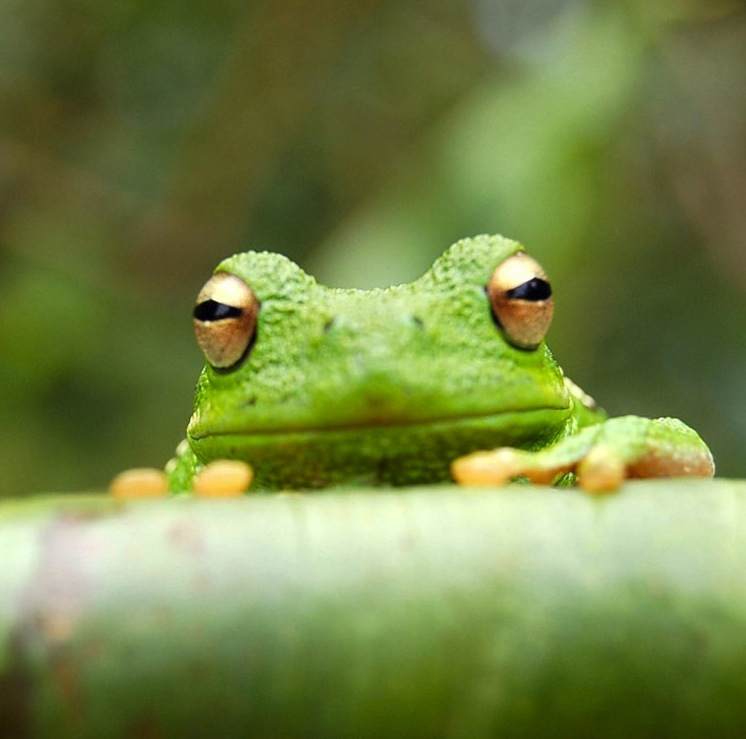
\includegraphics[height=6cm, width=8cm]{img/frog.jpg}
%     \caption{Caption (questo viene scritto nell'indice delle figure)}
%     % La label serve per riferirti all'immagine piu' avanti nel testo: \cref{fig:frog}
%     \label{fig:frog}
% \end{figure}

% \section{Tabelle}
% \subsection{Tabella semplice}
% Nota il modificatore \texttt{[H]}, la caption e la label.

% \begin{table}[H]
%     \centering
%     \begin{tabular}{|c|c|}
%     \hline
%         \textbf{Pratiche agili} & \textbf{Studenti}  \\ \hline
%         Sprint planning & 73  \\ \hline
%         Pair programming & 73  \\ \hline
%         Retrospettiva & 48  \\ \hline
%     \end{tabular}
%     \caption{Tabella semplice (anche questo viene scritto nell'indice delle tabelle)}
%     \label{tab:simple}
% \end{table}

% \subsection{Tabelle avanzate}
% Con \texttt{multirow} puoi fare righe piu' grandi del normale.

% \begin{table}[H]
%     \centering
%     \begin{tabular}{|c|c|c|c|c|}
%     \hline
%         \textbf{Team} & \textbf{LoC ver.} & \textbf{LoC svil.} & \textbf{Ore svil.} & \textbf{LoC/h}  \\ \hline
%         \multirow{2}*{1} & 1148 & m: 888  & m: 40 & 22\cr & Diff: $-$1852 & $\sigma$: 371 & $\sigma$: 27 & \\ \hline
%         \multirow{2}*{2} & 1858 & m: 1404 & m: 65 & 22\cr & Diff: $-$448  & $\sigma$: 1222 & $\sigma$: 78 & \\ \hline
%         \multirow{2}*{3} & 1640 & m: 1400 & m: 96 & 15\cr & Diff: $-$2810 & $\sigma$: 1417 & $\sigma$: 41 & \\ \hline
%     \end{tabular}
%     \caption{Tabella con multirow}
%     \label{tab:avanz}
% \end{table}

% \subsubsection{Tabelle girate}
% Se usi \texttt{landscape} la tabella viene girata (utile per tabelle molto larghe).
% \begin{landscape}
% \begin{table}[H]
%     \centering
%     \begin{tabular}{|c|c|}
%     \hline
%         \textbf{Numero} & \textbf{\#}  \\ \hline
%         UNO & 1  \\ \hline
%         DUE & 2  \\ \hline
%         TRE & 3  \\ \hline
%     \end{tabular}
%     \caption{Tabella girata}
%     \label{tab:girata}
% \end{table}
% \end{landscape}

% \section{Grafici con TikZ}
% Puoi creare grafici con \texttt{tikzpicture}.
% Tutorial completo: \url{https://tikz.dev/}

% % Esempio: assi cartesiani con range ragionevole (max x=10 per evitare overfull)
% \begin{tikzpicture}
%   \draw[->] (-0.5,0) -- (10,0) node[right] {$x$};
%   \draw[->] (0,-0.5) -- (0,5) node[above] {$y$};
%   \foreach \x in {1,2,...,9}
%     \draw (\x,-0.1) -- (\x,0.1) node[below] {\tiny\x};
%   \foreach \y in {1,2,3,4}
%     \draw (-0.1,\y) -- (0.1,\y) node[left] {\tiny\y};
%   \fill (0,0) circle[radius=2pt];
%   % Esempio di curva:
%   \draw[blue, thick, domain=0:9, samples=100] plot (\x, {0.5*\x});
% \end{tikzpicture}

% \section{Import di altri file .tex}
% Molto utile per capitoli separati:
% \begin{verbatim}
% % =============================================================================
% capitolo1_contesto.tex
% Capitolo 1: Contesto scientifico e tecnologico
%
% LINEE GUIDA VITALI:
%  Questo capitolo risponde alla domanda: "Perche' il problema non e' gia' risolto?"
%
%  A) STATO DELL'ARTE:
%     Descrivi gli approcci esistenti. Per ognuno: cosa fa bene, cosa fa male,
%     perche' non e' sufficiente.
%     CITAZIONI OBBLIGATORIE: ogni affermazione su lavori altrui vuole \cite{XYZ99}.
%     Esempio: "Come dimostrato da \citet{Tiz20}, l'approccio X ha il limite di..."
%
%  B) NUOVI STRUMENTI / ALGORITMI ABILITANTI:
%     Se il tuo lavoro sfrutta tecnologie recenti (LLM, nuovi framework, ecc.),
%     spiegale qui con sufficiente dettaglio da giustificare le scelte del Cap. 2.
%
%  C) IL GAP:
%     Concludi con una sintesi di cosa manca nello stato dell'arte
%     e come il tuo lavoro si posiziona per colmarlo.
%
%  REGOLA D'ORO: Non fare affermazioni senza fonte. Cita sempre con \cite{XYZ99}.
%  LUNGHEZZA SUGGERITA: 15-25 pagine.
% =============================================================================

% --- A. STATO DELL'ARTE ---
% Descrivi i principali approcci esistenti al tuo problema.
% Per ogni approccio: punti di forza, limiti, perche' non basta.

% --- B. TECNOLOGIE E STRUMENTI ABILITANTI ---
% Descrivi le tecnologie chiave su cui si basa il tuo prototipo.
% Spiega perche' le hai scelte rispetto ad alternative.

% --- C. GAP E MOTIVAZIONE ---
% Sintetizza: cosa manca nello stato dell'arte?
% Questa sezione prepara il lettore al Capitolo 2.

Scrivi qui il contenuto del capitolo 1 sul contesto scientifico.

% \end{verbatim}

% \section{Math mode}
% Inline: $5 \times \alpha = 3\lambda$

% Display:
% \[ \frac{\sum_{i=1}^{n} 3i\theta}{12k^2 \times 7} \]

% Numerata (con label):
% \begin{equation}
%     \frac{1}{2} \times A_{bcd} \times E^{fgh}
%     \label{eq:esempio}
% \end{equation}

% \section{URL e note a pie' di pagina}
% Per mettere un link usa \verb|\url{}|: \url{https://wikipedia.org}

% Per note a pie' di pagina usa \verb|\footnote{}|\footnote{Tipo questa.}

% \section{Code snippet}
% \begin{lstlisting}[language=C, caption={Hello World in C}, label={lst:helloC}]
% #include <stdio.h>

% int main(void) {
%     printf("Hello World\n");
%     return 0;
% }
% \end{lstlisting}

% \section{Verbatim}
% \begin{verbatim}
%     Qui puoi scrivere

%     come      vuoi
%     e viene tutto
% scritto monospaziato
% \end{verbatim}

% \section{Riferimenti incrociati}
% Le label servono per riferirti ad altre parti del testo.
% Esempio: ``vedi \cref{chap:intro}''.\\
% Con \texttt{cleveref} ottieni automaticamente la dicitura corretta:
% \cref{chap:intro}, \cref{tab:simple}, \cref{fig:frog}, \cref{eq:esempio}.

% \section{Citazioni}
% Per citare usa \verb|\cite{}| con la chiave del file \texttt{refs.bib}.
% Esempio:
% \begin{verbatim}
% ``come dimostrato da \citet{XYZ99}''
% \end{verbatim}

% Formati disponibili con \texttt{natbib}:
% \begin{itemize}
%     \item \verb|\cite{XYZ99}|  $\to$ [XYZ99]
%     \item \verb|\citet{XYZ99}| $\to$ Autore [XYZ99]  (in-text, soggetto della frase)
%     \item \verb|\citep{XYZ99}| $\to$ (Autore, Anno)  (parentetico)
% \end{itemize}

% Sostituisci \texttt{XYZ99} con la chiave della tua voce in \texttt{refs.bib}.

% %       nel file tesi.tex.
% % =============================================================================

% \section{Immagini}
% Quando usi \texttt{figure}, ricordati il modificatore di posizione tra quadre:
% \texttt{H} significa esattamente nel punto dove si trova nel file .tex (consigliato).

% \begin{figure}[H]
%     \centering
%     % Se metti solo una delle due dimensioni, l'altra scala in automatico.
%     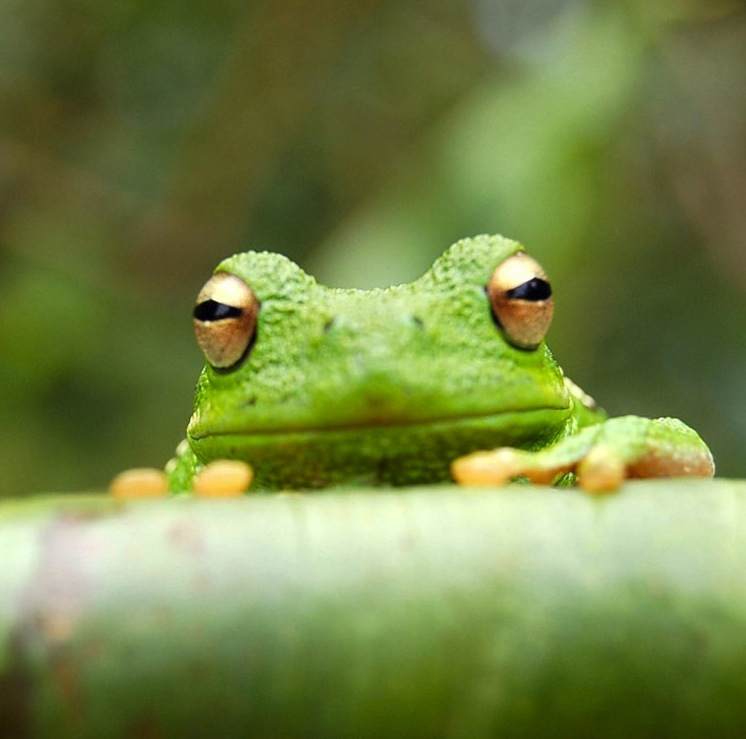
\includegraphics[height=6cm, width=8cm]{img/frog.jpg}
%     \caption{Caption (questo viene scritto nell'indice delle figure)}
%     % La label serve per riferirti all'immagine piu' avanti nel testo: \cref{fig:frog}
%     \label{fig:frog}
% \end{figure}

% \section{Tabelle}
% \subsection{Tabella semplice}
% Nota il modificatore \texttt{[H]}, la caption e la label.

% \begin{table}[H]
%     \centering
%     \begin{tabular}{|c|c|}
%     \hline
%         \textbf{Pratiche agili} & \textbf{Studenti}  \\ \hline
%         Sprint planning & 73  \\ \hline
%         Pair programming & 73  \\ \hline
%         Retrospettiva & 48  \\ \hline
%     \end{tabular}
%     \caption{Tabella semplice (anche questo viene scritto nell'indice delle tabelle)}
%     \label{tab:simple}
% \end{table}

% \subsection{Tabelle avanzate}
% Con \texttt{multirow} puoi fare righe piu' grandi del normale.

% \begin{table}[H]
%     \centering
%     \begin{tabular}{|c|c|c|c|c|}
%     \hline
%         \textbf{Team} & \textbf{LoC ver.} & \textbf{LoC svil.} & \textbf{Ore svil.} & \textbf{LoC/h}  \\ \hline
%         \multirow{2}*{1} & 1148 & m: 888  & m: 40 & 22\cr & Diff: $-$1852 & $\sigma$: 371 & $\sigma$: 27 & \\ \hline
%         \multirow{2}*{2} & 1858 & m: 1404 & m: 65 & 22\cr & Diff: $-$448  & $\sigma$: 1222 & $\sigma$: 78 & \\ \hline
%         \multirow{2}*{3} & 1640 & m: 1400 & m: 96 & 15\cr & Diff: $-$2810 & $\sigma$: 1417 & $\sigma$: 41 & \\ \hline
%     \end{tabular}
%     \caption{Tabella con multirow}
%     \label{tab:avanz}
% \end{table}

% \subsubsection{Tabelle girate}
% Se usi \texttt{landscape} la tabella viene girata (utile per tabelle molto larghe).
% \begin{landscape}
% \begin{table}[H]
%     \centering
%     \begin{tabular}{|c|c|}
%     \hline
%         \textbf{Numero} & \textbf{\#}  \\ \hline
%         UNO & 1  \\ \hline
%         DUE & 2  \\ \hline
%         TRE & 3  \\ \hline
%     \end{tabular}
%     \caption{Tabella girata}
%     \label{tab:girata}
% \end{table}
% \end{landscape}

% \section{Grafici con TikZ}
% Puoi creare grafici con \texttt{tikzpicture}.
% Tutorial completo: \url{https://tikz.dev/}

% % Esempio: assi cartesiani con range ragionevole (max x=10 per evitare overfull)
% \begin{tikzpicture}
%   \draw[->] (-0.5,0) -- (10,0) node[right] {$x$};
%   \draw[->] (0,-0.5) -- (0,5) node[above] {$y$};
%   \foreach \x in {1,2,...,9}
%     \draw (\x,-0.1) -- (\x,0.1) node[below] {\tiny\x};
%   \foreach \y in {1,2,3,4}
%     \draw (-0.1,\y) -- (0.1,\y) node[left] {\tiny\y};
%   \fill (0,0) circle[radius=2pt];
%   % Esempio di curva:
%   \draw[blue, thick, domain=0:9, samples=100] plot (\x, {0.5*\x});
% \end{tikzpicture}

% \section{Import di altri file .tex}
% Molto utile per capitoli separati:
% \begin{verbatim}
% % =============================================================================
% capitolo1_contesto.tex
% Capitolo 1: Contesto scientifico e tecnologico
%
% LINEE GUIDA VITALI:
%  Questo capitolo risponde alla domanda: "Perche' il problema non e' gia' risolto?"
%
%  A) STATO DELL'ARTE:
%     Descrivi gli approcci esistenti. Per ognuno: cosa fa bene, cosa fa male,
%     perche' non e' sufficiente.
%     CITAZIONI OBBLIGATORIE: ogni affermazione su lavori altrui vuole \cite{XYZ99}.
%     Esempio: "Come dimostrato da \citet{Tiz20}, l'approccio X ha il limite di..."
%
%  B) NUOVI STRUMENTI / ALGORITMI ABILITANTI:
%     Se il tuo lavoro sfrutta tecnologie recenti (LLM, nuovi framework, ecc.),
%     spiegale qui con sufficiente dettaglio da giustificare le scelte del Cap. 2.
%
%  C) IL GAP:
%     Concludi con una sintesi di cosa manca nello stato dell'arte
%     e come il tuo lavoro si posiziona per colmarlo.
%
%  REGOLA D'ORO: Non fare affermazioni senza fonte. Cita sempre con \cite{XYZ99}.
%  LUNGHEZZA SUGGERITA: 15-25 pagine.
% =============================================================================

% --- A. STATO DELL'ARTE ---
% Descrivi i principali approcci esistenti al tuo problema.
% Per ogni approccio: punti di forza, limiti, perche' non basta.

% --- B. TECNOLOGIE E STRUMENTI ABILITANTI ---
% Descrivi le tecnologie chiave su cui si basa il tuo prototipo.
% Spiega perche' le hai scelte rispetto ad alternative.

% --- C. GAP E MOTIVAZIONE ---
% Sintetizza: cosa manca nello stato dell'arte?
% Questa sezione prepara il lettore al Capitolo 2.

Scrivi qui il contenuto del capitolo 1 sul contesto scientifico.

% \end{verbatim}

% \section{Math mode}
% Inline: $5 \times \alpha = 3\lambda$

% Display:
% \[ \frac{\sum_{i=1}^{n} 3i\theta}{12k^2 \times 7} \]

% Numerata (con label):
% \begin{equation}
%     \frac{1}{2} \times A_{bcd} \times E^{fgh}
%     \label{eq:esempio}
% \end{equation}

% \section{URL e note a pie' di pagina}
% Per mettere un link usa \verb|\url{}|: \url{https://wikipedia.org}

% Per note a pie' di pagina usa \verb|\footnote{}|\footnote{Tipo questa.}

% \section{Code snippet}
% \begin{lstlisting}[language=C, caption={Hello World in C}, label={lst:helloC}]
% #include <stdio.h>

% int main(void) {
%     printf("Hello World\n");
%     return 0;
% }
% \end{lstlisting}

% \section{Verbatim}
% \begin{verbatim}
%     Qui puoi scrivere

%     come      vuoi
%     e viene tutto
% scritto monospaziato
% \end{verbatim}

% \section{Riferimenti incrociati}
% Le label servono per riferirti ad altre parti del testo.
% Esempio: ``vedi \cref{chap:intro}''.\\
% Con \texttt{cleveref} ottieni automaticamente la dicitura corretta:
% \cref{chap:intro}, \cref{tab:simple}, \cref{fig:frog}, \cref{eq:esempio}.

% \section{Citazioni}
% Per citare usa \verb|\cite{}| con la chiave del file \texttt{refs.bib}.
% Esempio:
% \begin{verbatim}
% ``come dimostrato da \citet{XYZ99}''
% \end{verbatim}

% Formati disponibili con \texttt{natbib}:
% \begin{itemize}
%     \item \verb|\cite{XYZ99}|  $\to$ [XYZ99]
%     \item \verb|\citet{XYZ99}| $\to$ Autore [XYZ99]  (in-text, soggetto della frase)
%     \item \verb|\citep{XYZ99}| $\to$ (Autore, Anno)  (parentetico)
% \end{itemize}

% Sostituisci \texttt{XYZ99} con la chiave della tua voce in \texttt{refs.bib}.

% %       nel file tesi.tex.
% % =============================================================================

% \section{Immagini}
% Quando usi \texttt{figure}, ricordati il modificatore di posizione tra quadre:
% \texttt{H} significa esattamente nel punto dove si trova nel file .tex (consigliato).

% \begin{figure}[H]
%     \centering
%     % Se metti solo una delle due dimensioni, l'altra scala in automatico.
%     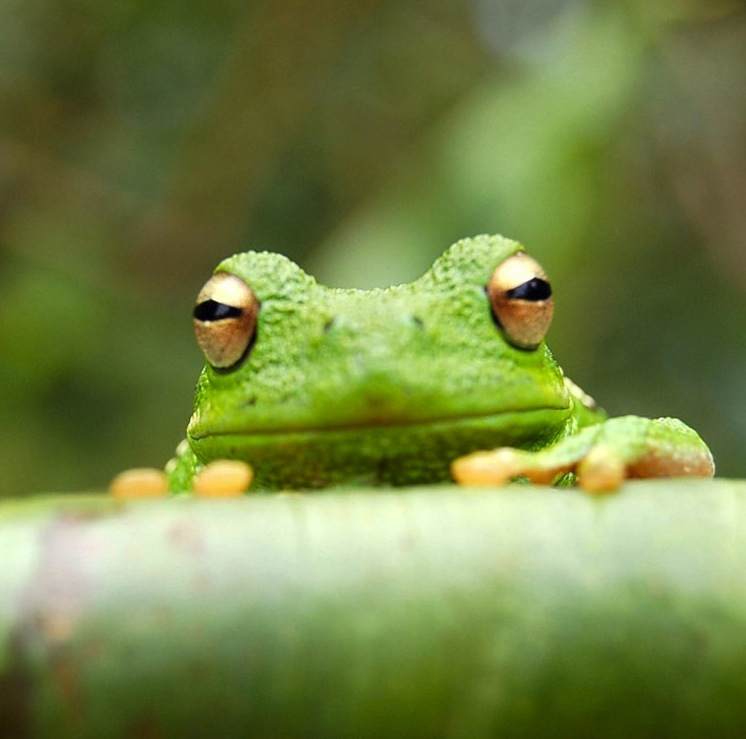
\includegraphics[height=6cm, width=8cm]{img/frog.jpg}
%     \caption{Caption (questo viene scritto nell'indice delle figure)}
%     % La label serve per riferirti all'immagine piu' avanti nel testo: \cref{fig:frog}
%     \label{fig:frog}
% \end{figure}

% \section{Tabelle}
% \subsection{Tabella semplice}
% Nota il modificatore \texttt{[H]}, la caption e la label.

% \begin{table}[H]
%     \centering
%     \begin{tabular}{|c|c|}
%     \hline
%         \textbf{Pratiche agili} & \textbf{Studenti}  \\ \hline
%         Sprint planning & 73  \\ \hline
%         Pair programming & 73  \\ \hline
%         Retrospettiva & 48  \\ \hline
%     \end{tabular}
%     \caption{Tabella semplice (anche questo viene scritto nell'indice delle tabelle)}
%     \label{tab:simple}
% \end{table}

% \subsection{Tabelle avanzate}
% Con \texttt{multirow} puoi fare righe piu' grandi del normale.

% \begin{table}[H]
%     \centering
%     \begin{tabular}{|c|c|c|c|c|}
%     \hline
%         \textbf{Team} & \textbf{LoC ver.} & \textbf{LoC svil.} & \textbf{Ore svil.} & \textbf{LoC/h}  \\ \hline
%         \multirow{2}*{1} & 1148 & m: 888  & m: 40 & 22\cr & Diff: $-$1852 & $\sigma$: 371 & $\sigma$: 27 & \\ \hline
%         \multirow{2}*{2} & 1858 & m: 1404 & m: 65 & 22\cr & Diff: $-$448  & $\sigma$: 1222 & $\sigma$: 78 & \\ \hline
%         \multirow{2}*{3} & 1640 & m: 1400 & m: 96 & 15\cr & Diff: $-$2810 & $\sigma$: 1417 & $\sigma$: 41 & \\ \hline
%     \end{tabular}
%     \caption{Tabella con multirow}
%     \label{tab:avanz}
% \end{table}

% \subsubsection{Tabelle girate}
% Se usi \texttt{landscape} la tabella viene girata (utile per tabelle molto larghe).
% \begin{landscape}
% \begin{table}[H]
%     \centering
%     \begin{tabular}{|c|c|}
%     \hline
%         \textbf{Numero} & \textbf{\#}  \\ \hline
%         UNO & 1  \\ \hline
%         DUE & 2  \\ \hline
%         TRE & 3  \\ \hline
%     \end{tabular}
%     \caption{Tabella girata}
%     \label{tab:girata}
% \end{table}
% \end{landscape}

% \section{Grafici con TikZ}
% Puoi creare grafici con \texttt{tikzpicture}.
% Tutorial completo: \url{https://tikz.dev/}

% % Esempio: assi cartesiani con range ragionevole (max x=10 per evitare overfull)
% \begin{tikzpicture}
%   \draw[->] (-0.5,0) -- (10,0) node[right] {$x$};
%   \draw[->] (0,-0.5) -- (0,5) node[above] {$y$};
%   \foreach \x in {1,2,...,9}
%     \draw (\x,-0.1) -- (\x,0.1) node[below] {\tiny\x};
%   \foreach \y in {1,2,3,4}
%     \draw (-0.1,\y) -- (0.1,\y) node[left] {\tiny\y};
%   \fill (0,0) circle[radius=2pt];
%   % Esempio di curva:
%   \draw[blue, thick, domain=0:9, samples=100] plot (\x, {0.5*\x});
% \end{tikzpicture}

% \section{Import di altri file .tex}
% Molto utile per capitoli separati:
% \begin{verbatim}
% % =============================================================================
% capitolo1_contesto.tex
% Capitolo 1: Contesto scientifico e tecnologico
%
% LINEE GUIDA VITALI:
%  Questo capitolo risponde alla domanda: "Perche' il problema non e' gia' risolto?"
%
%  A) STATO DELL'ARTE:
%     Descrivi gli approcci esistenti. Per ognuno: cosa fa bene, cosa fa male,
%     perche' non e' sufficiente.
%     CITAZIONI OBBLIGATORIE: ogni affermazione su lavori altrui vuole \cite{XYZ99}.
%     Esempio: "Come dimostrato da \citet{Tiz20}, l'approccio X ha il limite di..."
%
%  B) NUOVI STRUMENTI / ALGORITMI ABILITANTI:
%     Se il tuo lavoro sfrutta tecnologie recenti (LLM, nuovi framework, ecc.),
%     spiegale qui con sufficiente dettaglio da giustificare le scelte del Cap. 2.
%
%  C) IL GAP:
%     Concludi con una sintesi di cosa manca nello stato dell'arte
%     e come il tuo lavoro si posiziona per colmarlo.
%
%  REGOLA D'ORO: Non fare affermazioni senza fonte. Cita sempre con \cite{XYZ99}.
%  LUNGHEZZA SUGGERITA: 15-25 pagine.
% =============================================================================

% --- A. STATO DELL'ARTE ---
% Descrivi i principali approcci esistenti al tuo problema.
% Per ogni approccio: punti di forza, limiti, perche' non basta.

% --- B. TECNOLOGIE E STRUMENTI ABILITANTI ---
% Descrivi le tecnologie chiave su cui si basa il tuo prototipo.
% Spiega perche' le hai scelte rispetto ad alternative.

% --- C. GAP E MOTIVAZIONE ---
% Sintetizza: cosa manca nello stato dell'arte?
% Questa sezione prepara il lettore al Capitolo 2.

Scrivi qui il contenuto del capitolo 1 sul contesto scientifico.

% \end{verbatim}

% \section{Math mode}
% Inline: $5 \times \alpha = 3\lambda$

% Display:
% \[ \frac{\sum_{i=1}^{n} 3i\theta}{12k^2 \times 7} \]

% Numerata (con label):
% \begin{equation}
%     \frac{1}{2} \times A_{bcd} \times E^{fgh}
%     \label{eq:esempio}
% \end{equation}

% \section{URL e note a pie' di pagina}
% Per mettere un link usa \verb|\url{}|: \url{https://wikipedia.org}

% Per note a pie' di pagina usa \verb|\footnote{}|\footnote{Tipo questa.}

% \section{Code snippet}
% \begin{lstlisting}[language=C, caption={Hello World in C}, label={lst:helloC}]
% #include <stdio.h>

% int main(void) {
%     printf("Hello World\n");
%     return 0;
% }
% \end{lstlisting}

% \section{Verbatim}
% \begin{verbatim}
%     Qui puoi scrivere

%     come      vuoi
%     e viene tutto
% scritto monospaziato
% \end{verbatim}

% \section{Riferimenti incrociati}
% Le label servono per riferirti ad altre parti del testo.
% Esempio: ``vedi \cref{chap:intro}''.\\
% Con \texttt{cleveref} ottieni automaticamente la dicitura corretta:
% \cref{chap:intro}, \cref{tab:simple}, \cref{fig:frog}, \cref{eq:esempio}.

% \section{Citazioni}
% Per citare usa \verb|\cite{}| con la chiave del file \texttt{refs.bib}.
% Esempio:
% \begin{verbatim}
% ``come dimostrato da \citet{XYZ99}''
% \end{verbatim}

% Formati disponibili con \texttt{natbib}:
% \begin{itemize}
%     \item \verb|\cite{XYZ99}|  $\to$ [XYZ99]
%     \item \verb|\citet{XYZ99}| $\to$ Autore [XYZ99]  (in-text, soggetto della frase)
%     \item \verb|\citep{XYZ99}| $\to$ (Autore, Anno)  (parentetico)
% \end{itemize}

% Sostituisci \texttt{XYZ99} con la chiave della tua voce in \texttt{refs.bib}.
